\chapter{Preliminaries}

To understand this project and our contributions to the field, we will 
first present some background information about the topic, so that the reader 
can better understand both the problem and our proposed solutions.

\section{Terrains and Landscapes}

T
\subsection{General weathering effects}

\subsection{Freeze-thaw cycle}

\section{Terrain Representation and Modeling}
Virtual terrains are a fundamental aspect of this thesis, so it is important 
to review current approaches to represent and work with these types of models.
A deep dive into the state-of-the-art on terrain generation can be found on 
\cite{galin2019review}, but we are going to present only the most relevant 
methods for our project, as a full review is out of the scope of this thesis.

\subsection{Terrain Representations} \label{TerrainRep}

When representing terrains and landscapes there are multiple data structures 
and representations we can use depending on the ammount of information that 
we need to store and the nature of the model.

\vspace{10pt}

The main model representation techniques can be divided in \textit{Elevation
Models}, maninly focused on representing the surface of the terrain, and 
\textit{Volumetric Models}, that aim to capture some interal properties of 
the terrain as well as more complex structures.

\subsubsection{Elevation Models}
Elevation models are the simplest ways of representing virtual terrains. 
They consist on assigning an height to every point on a 2D space. In a more 
formal way, a terrain is represented by a function $h: \mathbb{R}^2 
\rightarrow \mathbb{R}$ that is at least $C^0$. From an height function we 
can easily extract the slope at one point $s(x,y)$ by using the norm of 
the gradient:

$$s(x,y) = \left \lVert \nabla h(x,y) \right \rVert = \left \lVert(\frac{\partial h}{\partial x}, \frac{\partial h}{\partial y}) \right \rVert$$

And from the gradient (projected to $\mathbb{R}^3$) we can easily obtain 
the normal at one point $n(x,y)$:

$$n(x,y) = \frac{(-\frac{\partial h}{\partial x}, -\frac{\partial h}{\partial y}, 1)}
{\left \lVert (-\frac{\partial h}{\partial x}, -\frac{\partial h}{\partial y}, 1)\right \rVert }$$

With the height, normal and slope we have all that we need for a basic 
representation of a terrain. Of course, as we are using a bivariate function
to represent the terrain, we can only have one elevation for each point 
on the domain, and that makes features like caves or overhangs impossible 
to represent with this method.

\vspace{10pt}

Despite its limitations, elevation models are widely used for its simplicity
and memory efficiency as they can capture the general structure of a landscape,
given that complex features like overhangs often represent a small part of the 
overall terrain.

\vspace{10pt}

To expand on this topic, elevation models only require a bivariate function
to represent the whole terrain, which can capture the whole terrain in a 
really simple closed-form expression, providing infinite precission with 
an extremly small ammount of memory. However, constructing functions that
represent complex realistic terrains is highly challenging and, for that 
reason, elevation models commonly use \textit{discrete heightfields} 
(also called \textit{Digital Elevation Models} or DEM) to represent terrains.

\vspace{10pt}

Discrete Heightfields are a collection of altitudes in a 2D grid. In order 
to create a DEM, you have to divide the domain of the terrain (assuming a 
rectangular domain) into a grid of $n x m$ cells, then, you assign an altitude
to every cell of the grid. The grid will only contain concrete values for
a set of discrete values, but you can obtain a height for every point of 
the domain by interpolating multiple values of the heightfield. This method
limits the accuracy of the model (as we stop having infinite precission), 
but it has the advantadge of representing arbitrary terrains in a really
simple way.

\vspace{10pt}

Heightfields are an extremly common way to represent terrains, and they can
be easily stored in textures and monochromatic images (as figure 
\ref{fig:anetoImage} shows), sometimes making use of the texture 
interpolation capabilities on the GPU to accelerate computations on 
heightfields. Specifically, DEMs are used on \cite{Argudo2025descriptors}, 
a project focused on terrain analysis that provides multiple metrics for 
terrains and whose code has been1 reutilized in this project to implement 
and test our erosion algorithm.

\begin{figure}
    \centering

    \subfigure[Aneto heightfield]{\label{fig:anetoTex}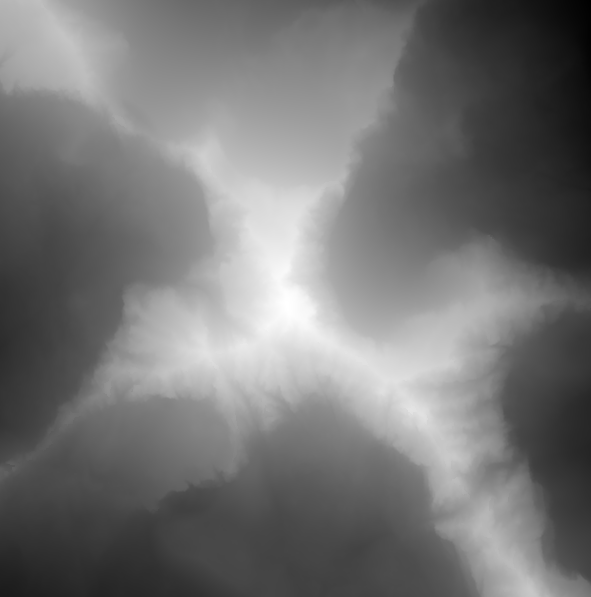
\includegraphics[width=0.28\linewidth]{Background/aneto.png}
    }
    \hspace{20pt}
    \subfigure[Aneto model on the app]{\label{fig:anetoApp}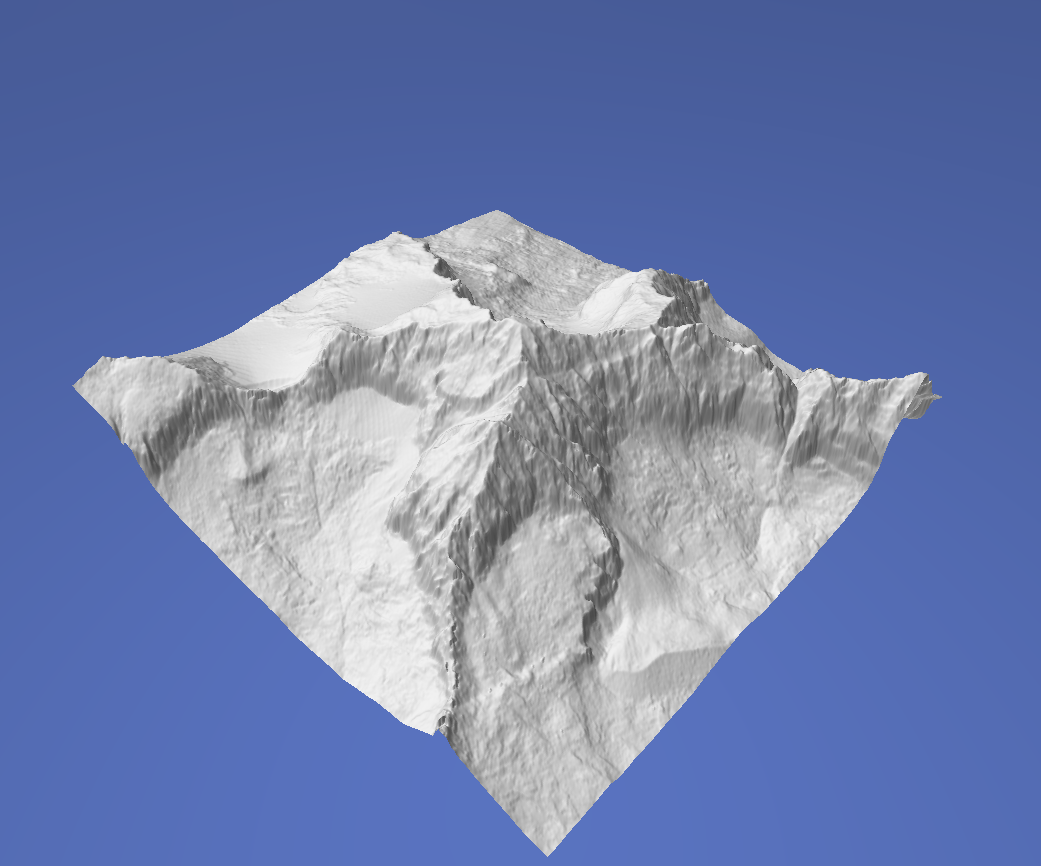
\includegraphics[width=0.335\linewidth]{Background/aneto-app.png}
        }
    
    \caption{Heightfield of the mountain Aneto as a monochromatic image and 
    the terrain produced by said heightfield on our application}
    \label{fig:anetoImage}
\end{figure}

To finalize the topic of elevation models, they have been extended to 
represent some internal structure of the model by employing a layered 
represesentation of the terrain. Layered representations are basically an 
ordered collection of height functions, each function representing a layer
of the model (which usually corresponds to a different material), resulting
in a stack of elevations for each grid cell. A representation of these 
types of layered heightfields can be seen on figure \ref{fig:layeredRep}

\begin{figure}
    \centering
    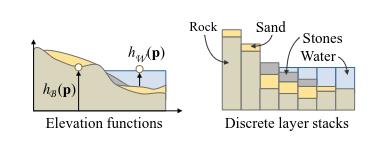
\includegraphics[scale=0.65]{Background/layeredRep.png}
    \caption{Illustration of stacked height functions,
    figure taken from \cite{galin2019review}}
    \label{fig:layeredRep}
\end{figure}

\vspace{10pt}

Layered representations have been used to simulate erosion (\cite{945341} 
and \cite{10.1145/3072959.3073667}) and, specially to simulate weathering 
events related to sediments as those types of rocks are naturally organized 
in layers. There are interesting works on this topics, but those will
be covered on chapter \ref{previousWork}

\subsubsection{Volumetric Models} 

As seen previously, layered representations are a way to represent 
different materials and properties of a terrains, but if we are really 
interested in encoding the internal structure of a landscape, we will 
have to use volumetric models. Volumetric models can be defined by a 
function $\mu: \mathbb{R}^3 \rightarrow \mathcal{M}$, where $\mathcal{M}$
denotes the set of materials used (air can count as a material). This 
function will be assigning every point of the 3D domain to a material, so
now complex structures like overhangs can be represented, as well as 
different internal compositions of the terrain.

\vspace{10pt}

Despite volumetric models being defined with a function, in practice we
will usually use a 3D grid with discrete samples and perform some
interpolation to obtain values outside the fixed grid points, similarlly
to what we did with DEMs. Each cell of the 3D grid is usually called a 
\textit{voxel} and the transformation of a model into a set of voxels a 
\textit{voxelization}. Voxelizations allow us to freely move and remove 
parts of the model, so they have potential to be used for algorithms that
change the structure of the landscape, like for erosion simulation, and 
they have been explored in the literature \cite{wingender2022simulation},
but they also have the huge drawback of being extremly expensive 
memory-wise. For that reason there has been a lot of work in the literature
making voxel representations more efficient (like adaptaive grids) or 
presenting novel ways to represent models encoding volumetric information.

\vspace{10pt}

For our purposes, we could have used a voxelization to implement our 
algorithm, but we decided that decomposing the terrain in voronoi cells 
would produce more natural results in a more efficient manner. The main 
concepts of the decomposition that we have chosen will be explained on 
section \ref{voronoiTheory}.

\subsection{Terrain Synthesis}

Terrain generation techniques can be divided in three main groups (although
it is common to employ methods from the three groups in the same project):

\begin{itemize}
    \item \textbf{Procedural Generation:} Procedural generation methods 
    artificially generate terrains from scratch by applying randomized 
    processes, like faulting or using noise. 
    \item \textbf{Example-based:} Example-based methods create virtual 
    terrains using scanned-data of real-world terrains.
    \item \textbf{Erosion Simulation:} Erosion simulations methods apply
    algorithms to simulate geomorphological processes when creating the 
    landscape.
\end{itemize}

Synthetic terrains usually can not represent all the complexity of a natural
landscape by procedural generation alone, and that is why erosion simiulations
are so important, not only in order to "predict" a future for the landscape 
but also to add realism on virtual terrains. Even example-based terrains
often fail to capture some aspects of the terrain they are trying to replicate, 
as scans have precission limitations (and the bigger the region you want 
to scan the more difficult it is to do it with accuracy), and erosion 
simulation can also intervene in those cases to add more complexity to 
the landscapes.

\section{Model Decompositions}
One of the core aspects of simluating erosion on 3D terrains is 
the model representation that we use. Any eroision simulation applied
on a 3D model will modfiy the model and its properties, so proper
data structures that allow for dynamic modifications of the model are 
key for these types of simulations. Additionally, applying erosion to an 
object also exposes the \textit{interior} of said object, so any model
representation that we use also has to encode some internal information of
the model, as internal points of a model might become part of the surface
at some point of the process.

\vspace{10pt}

In this section we are going to explain some of the decomopositons that 
can be applied to virtual terrains in order to convert the full model in 
a set of independent parts that can move freely to modify the overall 
landscape. We already mentioned voxalizations before 
(on section \ref{TerrainRep}), but due to voxelization limitations 
(mainly the memory cost), we explored more complex techniques to decompose
our models.

\subsection{Tetrahedralization}
As you might already know, every polygon can be divided into a set 
of trtiangles that exactly match the perimeter of the polygon. Triangulizations
can also be used to aproximate curved surfaces with arbitrary precission. 
In the case 3D polyhedra and volumes, tetrahedra are the equivalent of triangles,
we can aproximate any volume using terahedra, with more efficiency than 
with any other polyhedra (like cubes). 


\vspace{10pt}

We could use a tetrahedralization to decompose our terrain into tetrahedra and,
then apply our algorithm over those pieces, and we could even further divide 
the tetrahedra into more tetrahedra to adjust the granularity of the 
decomposition. The concept of tetrahedralization and tetrahedral meshas 
has been used to simulate erosion in the past \cite{turini2006simulating}, 
but we have chosen a differnt decomposition that has some advantadges over tetrahedralizations and produce more irregular 
shapes, which better represents the shapes we can observe in nature.

\begin{figure}
    \centering
    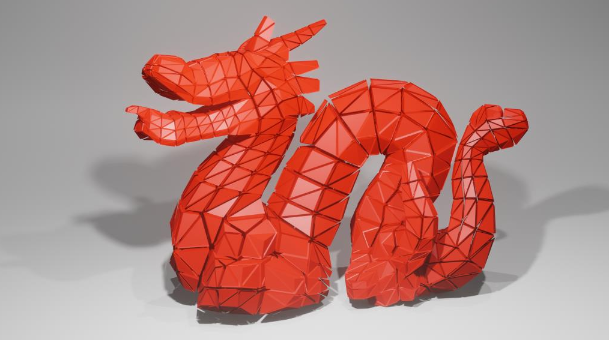
\includegraphics[scale=0.4]{Background/tetrahedralization.png}
    \caption{Example of a tetrahedalization, taken from \cite{Muller_2022}}
    \label{fig:tetrahedralization}
\end{figure}

\subsection{Voronoi Decomposition} \label{voronoiTheory}
Given a set of sample points, a voronoi decomposition is a partition of the space into 
multiple regions, where every region is defined by the set of all points 
that are closer to a given sample than any other sample. the boundary 
of every region (or cell), is given by the plane where every point of it
is at the same distance of two sample points.

\vspace{10pt}

In this thesis we decided to use voronoi cells for multiple reasons. First,
they can be generated with a lot of flexibility (just chose an arbitrary set 
of points) and we can adapt the decomposition depending on our needs. 
Additionally, the generated cells are not very regular, with varying 
sizes and shapes, which produces a more natural rocky appearance than
other more regular decompositions.

\begin{figure}
    \centering
    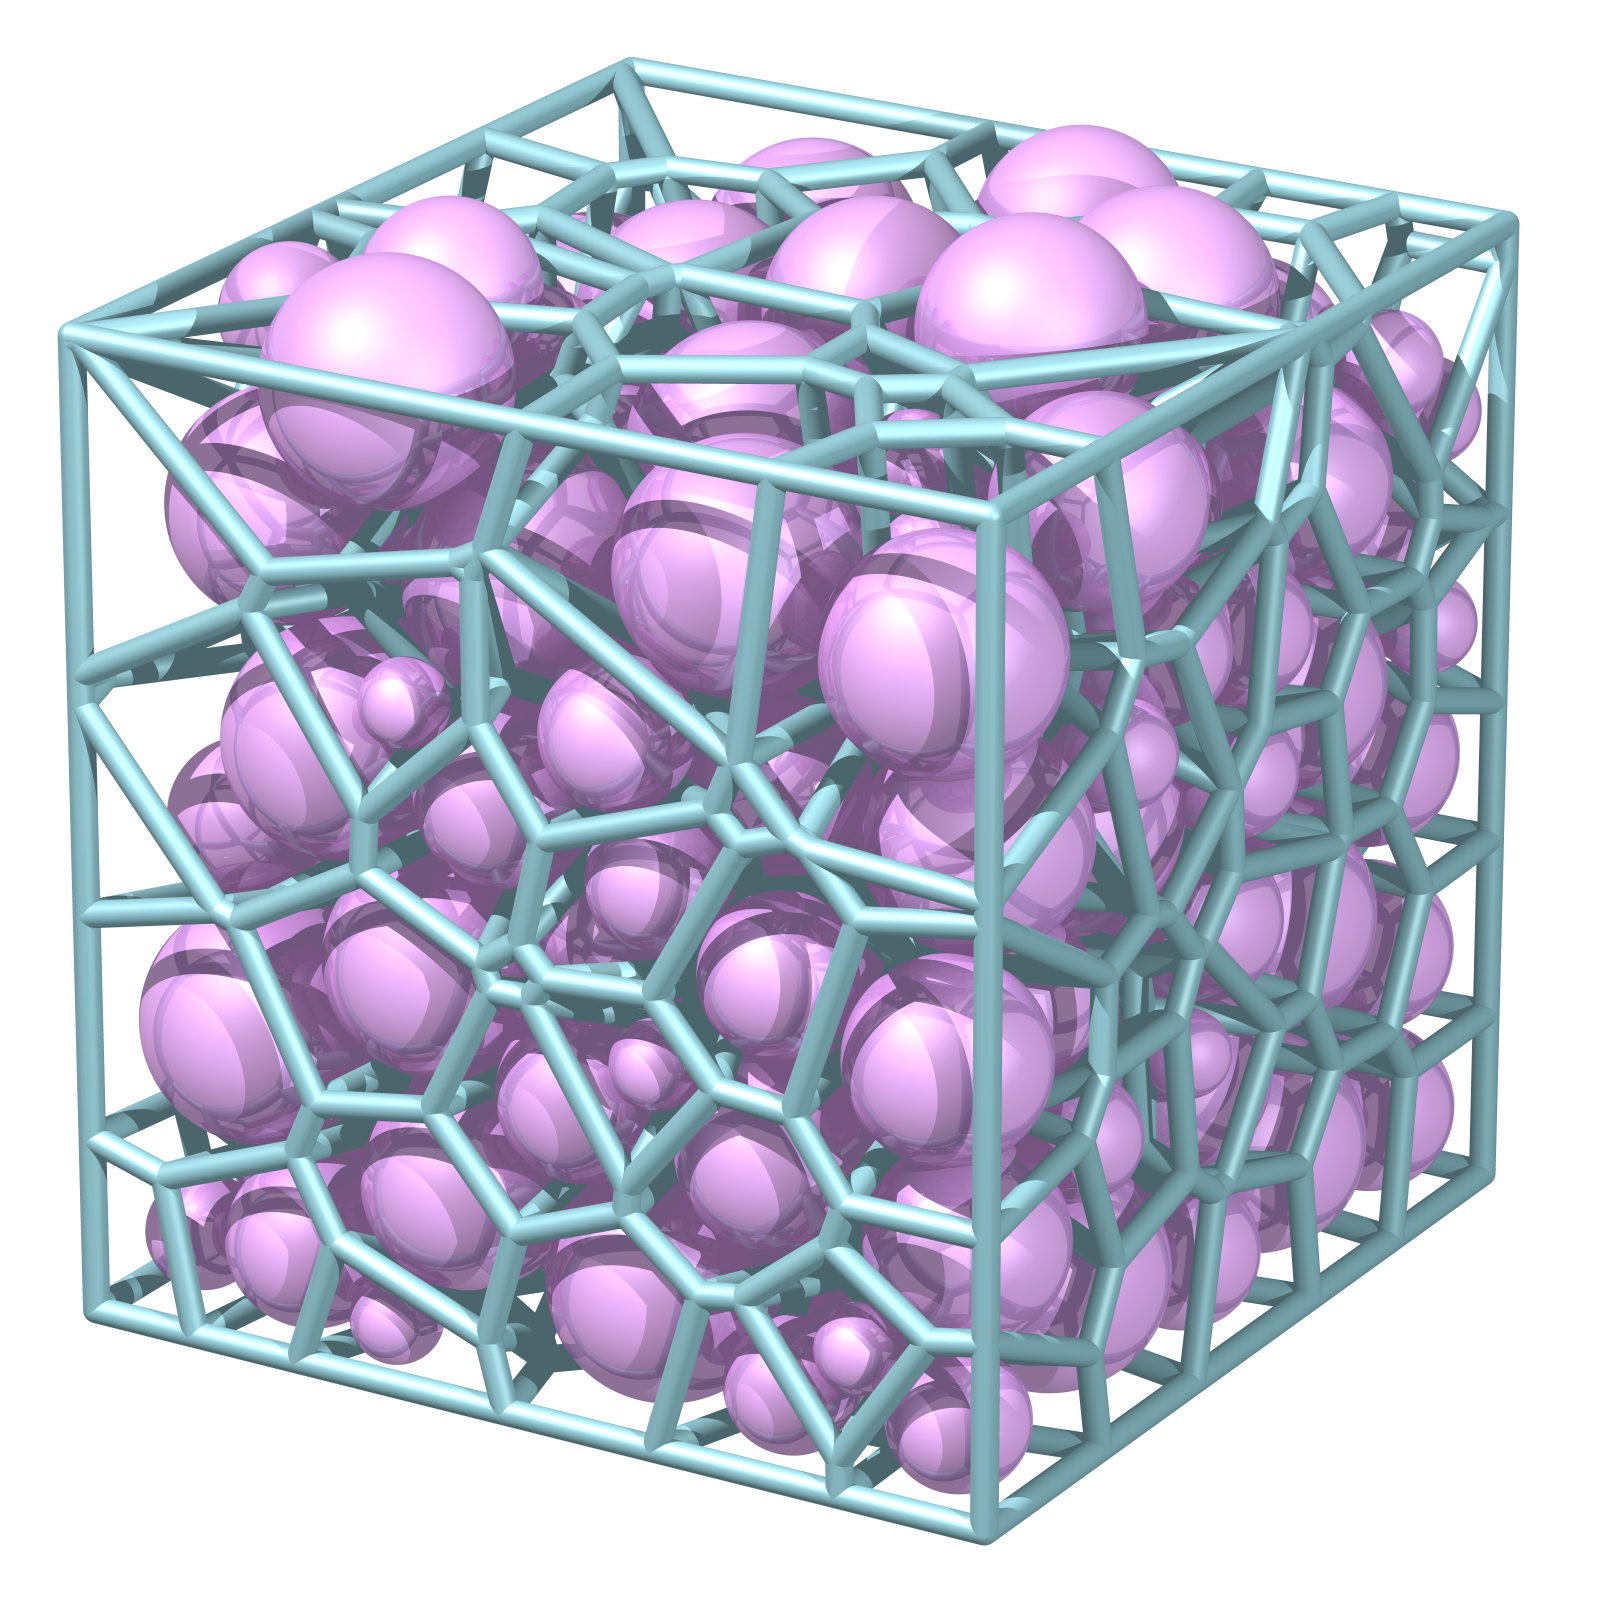
\includegraphics[scale=0.10]{Background/voronoiDecomp.png}
    \caption{Example of a voronoi decomposition of a cube, showing 
    the particles and faces of the decomposition. Figure taken 
    from the documentation of the C++ library Voro++ \cite{osti_code-54674}}
    \label{fig:voronoiDecomposition}
\end{figure}

\chapter{Previous Work} \label{previousWork}

There has been a multitude of proposed approaches to the problem of erosion 
simulation, each using different techniques and tackling different parts 
of the problem. To better understand our method and how it compares to 
previous solutions, we present a summary of the literature in the field, 
with their limitations and their differences with our approach. Additionally
we will also discuss the paper we are basing our algorithm on 
\cite{10.2312:ceig.20241139}, as our project can be seen as an extension to 
their work.

\section{Work in Applied sciences}
\subsubsection{Simulation of Crack propagation using eigenerosion}
\section{Work in Computer Graphics}
\subsection{Related Methods in Computer Graphics}

In this section we present work that is not focused on terrain erosion 
but it is still somewhat related to the topic.

\subsubsection{Spring-Mass Systems and Brittle Fracture}
Solid fracture is a fundamental aspect of simulating rock erosion, specially
when simulating the fractures caused by the infiltration of water and its 
freezing. To simulate breakage one common and simple approach is to use
spring-mass systems and remove overly extended springs. This approach was 
demonstrated years ago in \cite{10.1007/BF01900837} and \cite{10.1145/54852.378522}.

\vspace{10pt}

A more recent approach in this topic was presented in \cite{10.2312:sca.20141122},
where they explore the use of peridynamic systems for brittle fracture. 
Peridynamic systems are spring-mass systems with two particular properties:
they decouple stiffness from spring lenght and they also connect particles 
just by proximity instead of using 1-ring neighborhoods. An interesting 
part of the paper is that they have tried using Voronoi-Based Geometry 
to decompose the model and apply their spring-mass algorithm. In our case 
we also use voronoi-cells to generate our \textit{masses}, although the 
dynamics of the links and their fracture are different in our approach. 
Another approach that uses voronoi geometry for fracture can be found in 
\cite{10.1145/1242073.1242200}, although in this case they use voronoi polygons
over a surface instead of generating voronoi polyhedra in a volume.
\begin{figure}
    \centering
    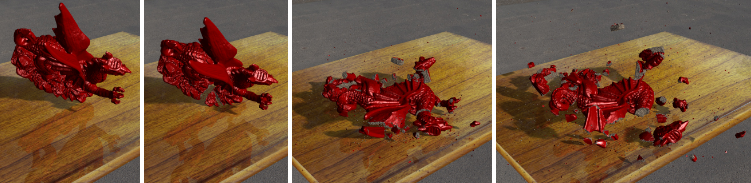
\includegraphics[scale=0.65]{Background/DragonBreak.png}
    \caption{A welsh dragon breaking. Taken from \cite{10.2312:sca.20141122}}
    \label{fig:dragonBreak}
\end{figure}
\subsubsection{Modeling Wood Decay}
Modeling realistic trees have some parallels to modeling terrains: The goal 
is to represent a complex natural object that is being constantly modified
through the interaction with its environment. Some work has been done \cite{10.1145/3641816}
\cite{10.1145/3721238.3730745} on simulating tree decay, which would be the equivalent of
simulating erosion on rocky terrains. 

\vspace{10pt}

On this specific topic, the recent work of \cite{YANG_SCHWARZ_2026} (which is yet
to be published on SIGGRAPH 2026) presents a really interesting method to 
simulate wood decay from fungal interaction. The method consists on 
dividing the tree model into \textit{segments} and then simulating a 
fungus infiltrating the host and generating fractures in the tree segments. 
A fungal infiltration also creates conditions facilitating further decay.
This is similar to the problem we are tackling: We divide a terrain into 
different components and then we simulate the water infiltrating the rock,
fracturing it and creating conditions where more water infiltration is 
favoured. The specific mechanics of rock fracture and wood decay are very 
different, so techniques for wood decay are not really applicable to our work, 
but the topic has interesting parallels.

\begin{figure}
    \centering
    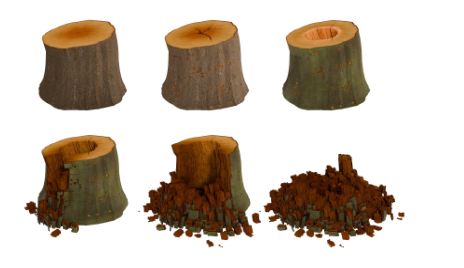
\includegraphics[scale=0.65]{Background/woodDecay.png}
    \caption{Example of wood dedcay of a cut tree trunk. Figure 
    taken from \cite{YANG_SCHWARZ_2026}}
    \label{fig:woodDecay}
\end{figure}
\subsection{Weathering in Computer Graphics}

Here we will show a summary of methods for erosion simulation in 
the literature.

\subsubsection{Physics-based Sandstone Simulator}

A recent approach to rock erosion was presented by \cite{10.1145/3731201}. The 
goal of the paper was to simulate sandstone dynamics with multiple effects like
wind and fluvial erosion. The presented method represents a sandstone structure 
using a set of particles and then they modify the model using the following 
equation for each particle:

$$\frac{\partial b}{\partial t} = -\varepsilon (\sigma_c) (\mathcal{W} + \mathcal{F})$$

Where $b$ represents the \textit{viability} which describes the 
expectancy that the rock has not been eroded, $\varepsilon$ represents 
the \textit{erodibility}, $\sigma_c$ is the Cauchy stress tensor, and 
$\mathcal{W} and \mathcal{F}$ represent the wind and fluvial local 
erosion effects. To compute that equation they divide te process into 
four parts: First they use the Material Point Method for stress computation 
and obtain $sigma_c$, then they compute the wind and fluvial erosion components, 
and finally they perform computations on deposition.

\vspace{10pt}

The problem solved by this simulator is similar to the one that we are 
tackling, but we are dealing with erosion by freezing and not with 
wind and fluvial erosion so our proposed solution will tackle other 
situations not covered by this method.


\begin{figure}
    \centering
    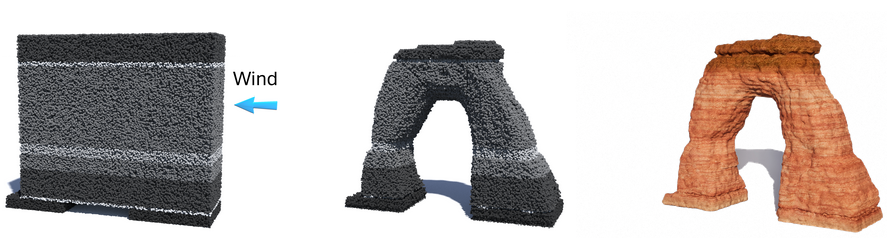
\includegraphics[scale=0.4]{Background/SandstoneArch.png}
    \caption{Arch produced by wind erosion. Figure taken from \cite{10.1145/3731201}}
    \label{fig:sandstoneArch}
\end{figure}


\subsubsection{Layered representations to simulate erosion}
In section \ref{TerrainRep} we briefly discussed layered heightfield 
represesentations andf how they can be used for erosion simulatio, 
specially to simulate sediments and their interactions. 
Using this strategy, the work of \cite{10.1145/3072959.3073667} presents an interesting approach, 
that specially focus in the interaction between vegetation and erosion and
their mutual interaction. In the paper, they divided the landscape in 
bedrock (unmoving), granular materials that may produce landslides and 
vegetation (dead and alive) and with that layered representation they could
run a simulation to modify those layers, representing the effect of 
erosion in the ecosystem, improving realism and showing the temporal 
evolution of a landscape. The layered representation they used can be 
appreciated on figure \ref{fig:layeredVeg}.

\vspace{10pt}

In our project we do not intend to deal with sediments and their interaction
with the environment, as the main erosion mechansim that we study is the 
one caused by water entering the pores of the rock and breaking them 
from inside, causing fractures and potentially separating chuncks of 
rocks from the main structure. Layered representations can represent
different features of the landscape with much more memory efficiency 
than other approaches and can also be used for erosion simulations, 
but they have limitations that make them not appropiate for certain 
types of erosion simulation, specially those that consider damage done 
on all the terrain and not just on the outer layers. 

\begin{figure}
    \centering
    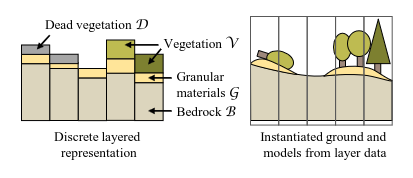
\includegraphics[scale=0.65]{Background/layeredVeg.png}
    \caption{Illustration of stacked height functions, used 
    to simulate interactions between vegetation and erosion. 
    figure taken from \cite{10.1145/3072959.3073667}}
    \label{fig:layeredVeg}
\end{figure}

\subsubsection{Machine Learning Approach}
In the field of terrain erosion there have also been approaches that use 
machine and deep learning to approximate the effect of erosion on a terrain 
and improve the realism of the landscape. In our work we do not use any of
these processes, so these methods are a little bit far of our proposed solution. 
Despite that, there are interesting solutions using this approach


\vspace{10pt}

In \cite{10.1145/3130800.3130804} they use a Conditional Generative Adversarial Network
trained on real-world terrain to add realistic detail to a rough sketch provided 
by the user, moreover, they also have a framework to simulate the evolution 
of the terrain through erosion (with another adversarial network); 
\cite{https://doi.org/10.1111/cgf.14992} presents an approach 
that procedually enhances terrains by adding erosion patterns using 
structured noise; and \cite{https://doi.org/10.1111/cgf.13345} uses Fully Convolutional Neural
Networks to upscale low-resolution terrains into plausible high-resolution 
ones.

\begin{figure}
    \centering
    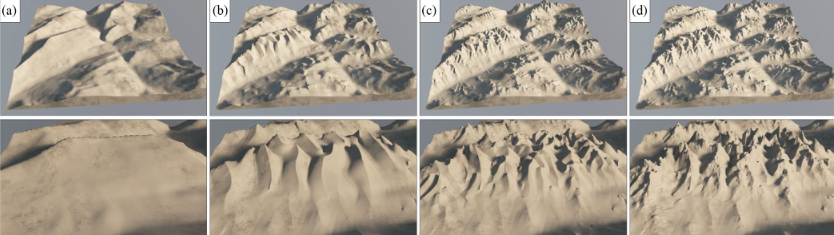
\includegraphics[scale=0.45]{Background/erosionDL.png}
    \caption{Example of terrain enhancenment through adding erosion patterns.
    Taken from \cite{https://doi.org/10.1111/cgf.14992}}
\end{figure}
\section{Base Simulator for this Project}

As mentioned on the introduction of this report (\ref{intro}), this thesis
is built upon the work of \cite{10.2312:ceig.20241139}, so we started from 
the algorithm they proposed and made some extensions and improvements. For 
this reason, in order to understand our projet we first have to understand
the method presented in the previous project.

\vspace{10pt}

In the paper, \cite{10.2312:ceig.20241139} present an approach to simulate
terrain erosion that can be divided into two main parts: first they divide 
the terrain into independent cells conected by \textit{links} between 
neighboring pieces, and, then, they apply an erosion algorithm to degrade 
the links and, eventually, remove the parts that have been disconnected 
from the terrain. Figure \ref{fig:waterInfiltration} shows the erosion 
simulation in action, with water infiltrating a terrain that has been 
decomposed into voronoi cells.

\vspace{10pt}

To perform the decomposition of the terrain into cells they sampled multiple
points of the model and then generated a voronoi tesellation. In our project
we still use the voronoi tesellation to generate the cell graph, but we 
modified the sampling to obtain better results. The original method used
boolean operations between the voronoi tesselation and the original model so
that the tesellation would fit the base terrain, but we tried to improve 
the decomposition so it could better fit the terrain without extra operations.


\vspace{10pt}

Regarding the algorithm that simulates water infiltration and link breakage, 
we implemented a mechanical model to represent link stress and modify 
those stress values once a link has been broken. This extension of the 
algorithm now modifies the state of the system after a fracture, instead 
of just modifying the state of one link, which can produce an effect called
crack propagation. The addition of this mechanical model makes the method 
more based in real natural processes and it improves its realism.

\vspace{10pt}

Additionally, we also experimented with multi-resolution decompositions in 
order to improve the efficiency of the simulation without compromising too
much on its quality. The algorithm can be applied in a less granular 
decomposition and then we can modify the more granular one according to the 
changes on the higher level.

\vspace{10pt}

Furthermore, this thesis also changes a lot the use tools and the testing 
framework. The original project implemented a blender plugin to demonstrate 
their solution, while we implemented the algorithm into a C++ OpenGL 
application.

\vspace{10pt}

Finally, even if the basic algortihm is taken from another project, we 
are going to explain in full detail all parts of the algorithm so that
the reader can understand our implementation just by reading this 
thesis. We are going to highlight our main contributions, but keep in 
mind some smaller details of the implementation may also be different 
to the original implementation (and we might not mention the change), 
as we took the main ideas of the method and implemented them in our own way.   
\begin{figure}
    \centering
    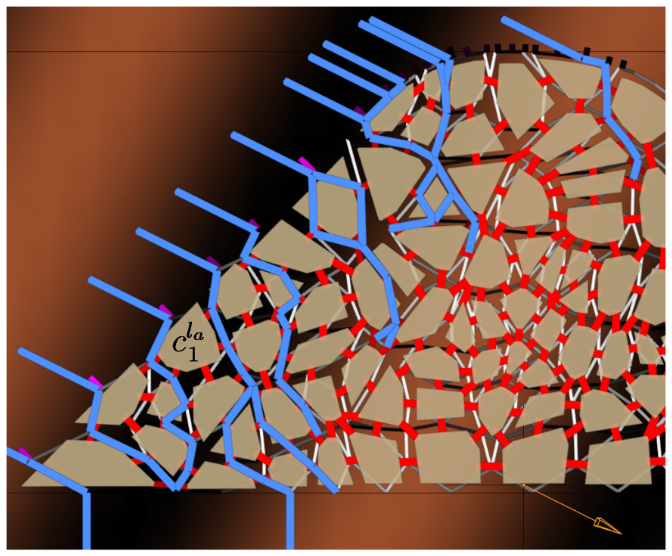
\includegraphics[scale=0.35]{Background/waterInfiltration.png}
    \caption{Example of water infiltrating a terrain divided into a set
    of voronoi cells connected by links. Taken from 
\cite{mateos_arlanzon_2023}}
    \label{fig:waterInfiltration}
\end{figure}


